\documentclass[a4paper]{article}

\usepackage{INTERSPEECH2018}
\usepackage{subfigure}

\title{AISHELL-2: Transforming Mandarin ASR Research Into Industrial Scale}
\name{Jiayu Du$^1$, Hui Bu$^2$}
%The maximum number of authors in the author list is twenty. If the number of contributing authors is more than twenty, they should be listed in a footnote or in acknowledgement section, as appropriate.
\address{
  $^1$AISHELL foundation$^*$\thanks{* AISHELL foundation is a non-profit online organization, dedicated to pushing forward speech industry via open-sourcing database to research institutes and contributing codes to open-source speech community.} \\
  $^2$Beijing Shell Shell Technology Co. Ltd., Beijing, China}
\email{aishell.foundation@gmail.com, buhui@aishelldata.com}

\begin{document}

\maketitle
%
\begin{abstract}
AISHELL-1 is by far the largest open-source speech corpus available for Mandarin
speech recognition research. It was released with a baseline system containing
training and testing pipelines for Mandarin ASR. In AISHELL-2, 1000 hours of
clean read-speech data from iOS is published, which is free for academic usage. On top of
AISHELL-2 corpus, an improved recipe is developed and released, containing key
components for industrial applications, such as Chinese word segmentation,
flexible vocabulary expension and phone set transformation etc. 
Pipelines support various state-of-the-art techniques, such
as time-delayed neural networks and Lattic-Free MMI objective funciton. 
In addition, we also release dev and test data from other channels(Android and Mic). 
For research community, we hope that AISHELL-2
corpus can be a solid resource for topics like transfer learning and robust
ASR. For industry, we hope AISHELL-2 recipe can be a helpful reference for
building meaningful industrial systems and products.
\end{abstract}
\noindent\textbf{Index Terms}: Speech recognition, Mandarin ASR, Industrial Speech Recognition

\section{Introduction}

Speech recognition (ASR) is one of the key techniques in the bloom of artificial
intelligence (AI). A lot of efforts has been made in both research and industry
to improve system performance. Among all efforts, deep learning has dominated
speech recognition in the recent half decade. One advantage of deep learning
frameworks is that neural network (NN) models turn out to be more robust when
more data is provided. Fortunately, along with the wide adoption of smart
phones, and the emerging market of various smart devices, real data from
applicational scenario are generated world-widely and everyday. Therefore,
collecting data becomes much easier than ever before for speech industry.

However, the research community have very limited access of real-world
application data. This is particularly true for Mandarin ASR, and many research
efforts do not scale well for industrial applications. In the field of computer
vision, there are many high quality free data sets which transform many research
efforts into industrial applications, such as ImageNet~\cite{imagenet} and
COCO~\cite{coco}. However, in the field of Mandarin ASR, there was no free
corpus with sufficient amount of high quality speech data to build a meaningful
research baseline, until the release of AISHELL-1~\cite{aishell1}. It contains
170 hours of Mandarin speech with high quality human transcriptions. In
addition, training and evaluation recipes for speech recognition and speaker
recogntion are released based on Kaldi~\cite{kaldi}. To the authors knowledge,
it has helped researchers who need high quality Mandarin speech corpus all over
the world~\cite{do2017}.

% Another issue with the Mandarin speech recognition research is that, there is
% still gap between a research prototype for demonstration and a working system
% for application. The open-source movement improves the transparency and
% availability of many research achievements. However, the attemp of direct
% deployment of a working system from an open-source demostration often fail. The
% effort of knowledage transfering from the research topic to application domain
% is enourmously high, and is normally off the record.

In this paper, we introduce AISHELL-2 corpus and AISHELL-2 recipe, as a complete 
self-contained baseline for industrial-scale Mandarin ASR research. 
Firstly, AISHELL-2 contains 1000 hours of clean read-speech data, which is free 
for academic usage. Secondly, an improved speech recognition
recipe is published, it contains must-have components for Mandarin ASR,
such as Chinese word segmentation, and a new design for customizable Chinese
lexicon, etc. Moreover, AISHELL-2 release dev and test data from different acoustic channels(Android and Mic),
these should be fruitful resources for transfer learning and robust ASR research.

This paper is organized as below. Section 2 introduces the structure and
specifications of the AISHELL-2 corpus. Section 3 describes the AISHELL-2
baseline recipe, including data preparation, GMM training, DNN training.
Section 4 presents baseline system evaluation results.

\section{The AISHELL-2 corpus}

The AISHELL-2 corpus contain 1000 hours of clean speech. The raw data were
recorded in a multi-channel manner with three kinds of devices, including a high
fidelity microphone, Android phones and iPhones. The relative position of
speaker and devices are shown in Figure~\ref{fig:setup}. Eventually, iPhone data
is open-sourced in AISHELL-2. Speaker, environment and content coverage are
fully considered as explained below
\begin{itemize}
\item 1991 speakers participated in the recording, including 845 male speakers
  and 1146 female speakers. Age of speaker ranges from 11 to over 40. Although
  only Mandarin speakers are selected, there are still some accent to some
  extent. 1293 speakers use a Northern accent, 678 speakers use a Southern
  accent and 20 speakers use other accent.
\item 1347 speakers are recorded in a studio, while the rest are recorded in a
  living room with natural reverberance.
\item The content of the recording prompt covers 8 major topics, including voice
  commands (such as IoT device control and digital sequence), place of interest,
  entertainment, finance, technology, sports, English spellings and free text
  without specific topic. The total number of prompts is around half a million.
\end{itemize}

\begin{figure}[t]
  \centering
  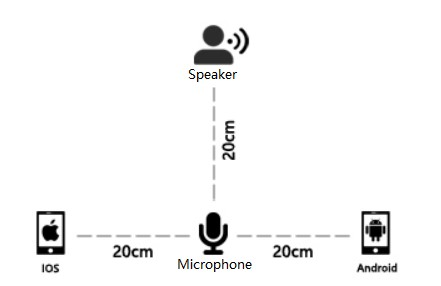
\includegraphics[width=\linewidth]{setup.jpg}
  \caption{Recording setup}
  \label{fig:setup}
\end{figure}

Besides the AISHELL-2 training corpus, we also provide develop and test
sets. The dev set contains 2500 utterances from 5 speakers, and the test set
contains 5000 utterances from 10 speakers. Each of the speaker contributed
approximately half an hour of voice, covering 500 prompts. First 7 prompts of
all speakers are sampled from a shared prompt pool extracted from high frequency
online queries. Speaker genders are covered.

\section{The AISHELL-2 recipe}

Based on AISHELL-2 corpus, a baseline Kaldi recipe is developed, including
data processing, acoustic model and language model
training, test set evaluation.

\subsection{Lexicon and word segmentation}

Different from English system, Mandarin ASR systems require word
segmentation. In AISHELL-1, word segmentation was implemented via forward
maximum matching algorithm[Ref], based on a variation of open-source mandarin
dictionary CC-CEDIT\footnote{https://cc-cedict.org/wiki}. In AISHELL-2, an
open-source Chinese dictionary called DaCiDian is
released\footnote{https://github.com/aishell-foundation/DaCiDian}. In most
common Chinese dictionaries, words are directly mapped to phonemes. While in
DaCiDian, this mapping is decomposed into 2 independent layers. An examplar
DaCiDian structure is shown in Figure~\ref{fig:lex1} and Figure~\ref{fig:lex2}.

\begin{itemize}
\item The first layer maps word to PinYin syllables~\cite{pinyin}. Anyone who is
  familiar with PinYin (basically every Mandarin speaker), can enrich DaCiDian's
  vocabulary by adding new words into this layer.
\item The second layer is a mapping from Pinyin syllable to phoneme. ASR system
  developers can easily adapt DaCiDian to their own phone set by redefining this
  layer of mapping.
\end{itemize}

\begin{figure}[t]
  \centering
  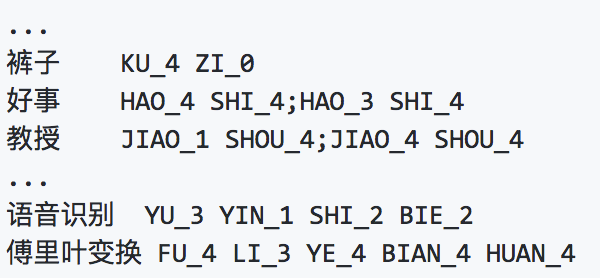
\includegraphics[width=0.8\linewidth]{dacidianl1.png}
  \caption{Layer 1 of DaCiDian}
  \label{fig:lex1}
\end{figure}
\begin{figure}[t]
  \centering
  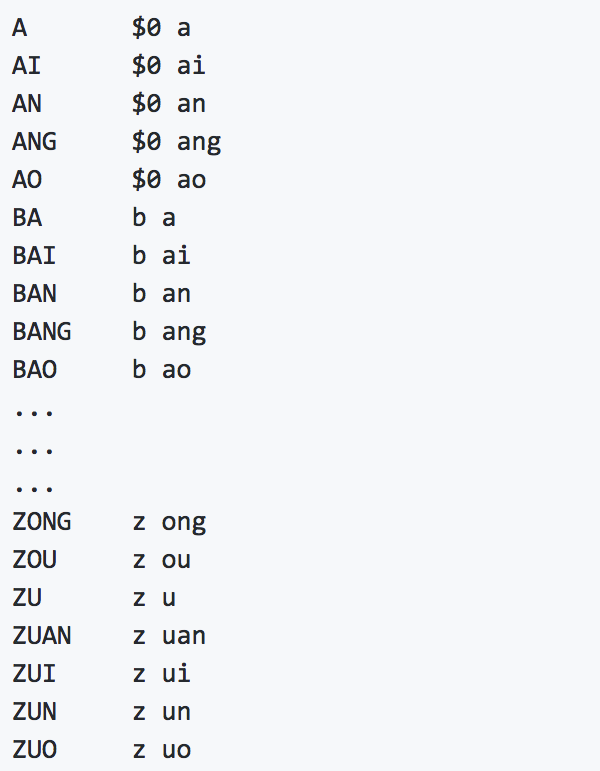
\includegraphics[width=0.8\linewidth]{dacidianl2.png}
  \caption{Layer 2 of DaCiDian}
  \label{fig:lex2}
\end{figure}

In terms of word segmentation, we choose a popular and easy-to-use open-source
toolkit called Jieba~\cite{jieba}, it implements a trie-tree based algorithm and
supports vocabulary customization.  Base on DaCiDian and Jieba, we provide a
script to segment AISHELL-2 acoustic data transcription and language model text.

\subsection{Acoustic model}

Two versions of the acoustic model training pipelines are provided, including
the GMM training based on maximum likelihood and the hybrid DNN-HMM training
based on cross entropy.

The GMM models are trained using 13 dimensional MFCCs. For sake of real time
demonstration, pitch is not included as acoustic feature. The training contains
four steps. A monophone model is trained to set a starting point for the
triphone models. A small triphone model and a larger triphone model are
consecutively trained using delta features. After that, a more sophisticated
feature transform method is applied to replace the delta features. Linear
discriminant analysis (LDA) is applied on a stack of frames to reduce the
dimension and MLLT based global transform is estimated iteratively. This is a
standard setup in Kaldi recipes. The resulting number of physical GMMs of the
four steps are 605, 3216, 5720 and 8080 respectively.

GMM training of the AISHELL-2 terminates at the speaker independent stage
without speaker dependent transform, such as fMLLR. From privacy point of view,
it is impractical to use customers' personal data and account
infomation. From architecture point of view, deploying a large scale
speaker-dependent commercial system is complex and costly. Therefore, AISHELL-2
adopts speaker independent GMM training. Moreover, it's not worth 
spending too much time and computation power in GMM stage, since the final system 
performance primarily depends on later NN models.

TODO update NN AM topo and training description here

% Neural network acoustic models are trained using 80 dimensional filter bank
% features. A time-delay neural network (TDNN) with 4 time-delay layers and 2
% full-connect layers is trained using batch normalization~\cite{tdnn}. All of the
% layers use 850 output RELU neurons~\cite{relu}. A recurrent neural network with
% 3 LSTM layers is trained using chunked BPTT with a output delay factor of
% 5~\cite{lstm}. Each of the LSTM layers contains 1024 cells and a projection of
% 256 output neurons~\cite{lstmp}.

\subsection{Language model}

A trigram language model is trained on 5.7 million words of the training
scripts. Out-of-vocabulary (OOV) words are mapped into $<$UNK$>$. The language
model is trained using Kneser-Ney smoothing and the final model has 516552
unigrams, 1498603 bigrams and 932475 trigrams.

\section{Evaluations}

The presented baseline system is trained on a standalone server with ordinary
configurations. The CPU is Intel Xeon processor of 2.3GHz and the GPUs are four
Nvidia Titan Xp. Character Error Rate (CER) is used as evaluation metric. 
The results along with the total training time of each model are presented in Table~\ref{tab:base}. 
Note that during training we only use iOS data for acoustic modeling, but we evaluate
these models on dev and test sets for all 3 channels(Android, Mic, and iOS). As
expected, system performance on iOS outperforms Android and Mic, due to better
acoustic channel matching between training and testing.

TODO update "improved" recipe result, including results on iOS, Android and Mic

\begin{table*}[th]
  \caption{Baseline system results and training time}
  \label{tab:base}
  \centering
  \begin{tabular}{ llllllll }
    \toprule
    CER               &  dev\_android           &  dev\_ios           &  dev\_mic           & test\_android            &  test\_ios           &  test\_mic          &  Training time         \\
    \midrule
    Monopphone        &  55.10                 &  50.85             &  54.95             &  51.35                  &  50.14              &  50.03             &  0.5                   \\
    Small triphone    &  32.66                 &  27.70             &  31.47             &  30.33                  &  27.90              &  28.76             &  1                     \\
    Large triphone    &  30.71                 &  25.72             &  29.18             &  28.26                  &  26.12              &  26.81             &  2                     \\
    LDA+MLLT          &  26.32                 &  22.29             &  25.34             &  24.44                  &  22.48              &  23.16             &  2.3                   \\
    TDNN              &  15.04                 &  11.75             &  16.96             &  12.78                  &  11.18              &  14.92             &  20                    \\
    LSTM              &  13.27                 &  10.81             &  13.65             &  11.91                  &  10.34              &  13.4              &  NA                    \\
    \bottomrule
  \end{tabular}
\end{table*}

\begin{table*}[th]
  \caption{Transfer learning results}
  \label{tab:trans}
  \centering
  \begin{tabular}{ lllllll }
    \toprule
    CER               &  dev\_android           &  dev\_ios           &  dev\_mic           &  test\_android           &  test\_ios           &  test\_mic     \\
    \midrule
    Baseline          &  15.04                 &  11.75             &  16.96             &  12.78                  &  11.18              &  14.92        \\
    Channel transfer  &  12.88                 &  12.16             &  12.13             &  11.65                  &  11.48              &  10.79        \\
    Domain transfer   &  8.07                  &  6.65              &  9.16              &  6.65                   &  5.63               &  8.05         \\
    Combined transfer &  6.66                  &  6.43              &  6.21              &  5.97                   &  5.77               &  5.48         \\
    \bottomrule
  \end{tabular}
\end{table*}

% \section{Customizing a speech recognition system}
% 
% One major barrier that stops the transforming from research prototypes into
% industrial applications is the scale of training data. Now that AISHELL-2 corpus
% and baseline system have been released, the potential of transforming the
% Mandarin ASR research into industrial scale can be fully discovered by
% customizing a speech recognition system based on the AISHELL-2
% baseline. Customizing a speech recognition system requires transferring the
% knowledge of a baseline system into a specific scenario which suits the target
% application. The knowledge include the channel through which the speech data is
% collected, and the language domain context of target applications.
% 
% \subsection{Acoustic channel fine-tuning}
% 
% Table~\ref{tab:base} shows that channel mismatch introduces significant
% performance decay. To alleviate this type of problem, various adaptation and
% transfer learning techniques have been proposed, depending on the amount of
% available matched data~\cite{adapt}. In AISHELL-2, we experiment the most
% straight forward method - acoustic model finetuning. A finetune recipe is
% provided, which takes matched data and mismatched model as input, and produces
% adapted model that suits the target channel. In the experiment, 100 hours of
% data from the mic channel is forced-aligned and fed into the baseline TDNN model
% (trained with ios data) via standard back-propagation, and results are shown in
% Table~\ref{tab:trans}. By transferring the channel of acoustic model, the
% performance on the matched subset, a.k.a. the mic subset, is significantly
% improved. Meanwhile, there is slight regression of the performance on the
% android subset. The performance on the android subset is also improved, which
% might due to better robustness of the acoustic model.
% 
% \subsection{Language domain adaptation}
% 
% The domain of language model is also crucial for applicational ASR
% systems. LM training text of AISHELL-2 are mostly collected from smart-home
% domain. In order to demonstrate domain transfer, we delibrately designed dev and
% test sets from general domain, then we collected 3 million sentences in addition
% (approximately 100 megabytes of text) from same domain as dev and test sets. The
% texts are segmented using the method as in Section 3.1. A trigram is estimated
% using modified Kneser-Ney smoothing~\cite{kn} and interpolated with the
% baseline LM using a weight of 0.5. During evaluation, the baseline AM is coupled
% with this interpolated LM. Table~\ref{tab:trans} shows that, by applying domain
% transfer, CER is decreased by approximately 45\% on all the subsets.
% 
% Furthermore, we combined the finetuned AM with the interpolated LM. The results
% are shown in the last row of Table~\ref{tab:trans}. The CER of all subsets for
% all channels are further decreased to around 6\%, suggesting that the robustness
% and performance of the baseline system is significantly improved via simple
% acoustic and language model transfer learning.

\section{Conclusions}

In this paper, AISHELL-2 Mandarin corpus and AISHELL-2 recipe are released,
freely available to research community, for building industrial scale research
baselines. We hope this open-source project may provide essential gradients for
researchers to explore more scalable techniques regarding to industrial
issues. 

\section{Acknowledgements}

The authors thank all the members of AISHELL foundation who contributed to this
project.

\bibliographystyle{IEEEtran}

\bibliography{mybib}

% \begin{thebibliography}{9}
% \bibitem[1]{Davis80-COP}
%   S.\ B.\ Davis and P.\ Mermelstein,
%   ``Comparison of parametric representation for monosyllabic word recognition in continuously spoken sentences,''
%   \textit{IEEE Transactions on Acoustics, Speech and Signal Processing}, vol.~28, no.~4, pp.~357--366, 1980.
% \bibitem[2]{Rabiner89-ATO}
%   L.\ R.\ Rabiner,
%   ``A tutorial on hidden Markov models and selected applications in speech recognition,''
%   \textit{Proceedings of the IEEE}, vol.~77, no.~2, pp.~257-286, 1989.
% \bibitem[3]{Hastie09-TEO}
%   T.\ Hastie, R.\ Tibshirani, and J.\ Friedman,
%   \textit{The Elements of Statistical Learning -- Data Mining, Inference, and Prediction}.
%   New York: Springer, 2009.
% \bibitem[4]{YourName17-XXX}
%   F.\ Lastname1, F.\ Lastname2, and F.\ Lastname3,
%   ``Title of your INTERSPEECH 2018 publication,''
%   in \textit{Interspeech 2018 -- 19\textsuperscript{th} Annual Conference of the International Speech Communication Association, September 2-6, Hyderabad, India Proceedings, Proceedings}, 2018, pp.~100--104.
% \end{thebibliography}

\end{document}
